\graphicspath{{chapters/_resources/}}

\chapter{Targeting transcription in cancer}
In order to perform transcription targeting in cancer, we first need to understand which genes are driving tumorigenesis.

\hypertarget{age-related-remodellling-of-oesophageal-epithelia-by-mutated-cancer-drivers}{%
\subsubsection{\texorpdfstring{Age-related remodellling of \textbf{oesophageal epithelia by mutated cancer drivers}}{Age-related remodellling of oesophageal epithelia by mutated cancer drivers}}\label{age-related-remodellling-of-oesophageal-epithelia-by-mutated-cancer-drivers}}

Biopsies from cancer (red) and non-cancer (green) sites from 58 y.o. male with risk for esophagus cancer (smoking and drinking heavily). By looking at the mutational burden, cancer samples has a higher MCF (mutant cell fraction). The normal biopsies showed several mutations too. If we look closer, mutations are hitting driver genes e.g.~NOTCH, TP53. Cancer samples' mutations are overlapping to a good extent and are present at a higher degree. In normal tissues we have \emph{independent mutations,} which suggests that independent clones are present in a normal epithelium.

\begin{figure}
\centering
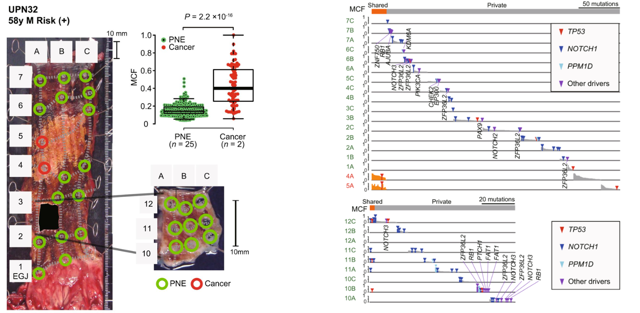
\includegraphics[width=0.5\textwidth]{../_resources/Screen_Shot_2022-11-04_at_10-50-01.png}
\caption{Yokoyama et al., Nature 2019}
\end{figure}

Yokoyama et al., Nature 2019

Divide patient samples in low and high risk, in normal tissues. The number of mutations per sample increases with risk and over time. By analyzing the mutation, 4 mutational signatures were identified: e.g.~APOBEC is responsible for globulin production, should be restricted to lymphocytes , C$\rightarrow$T mutation.

\begin{figure}
\centering
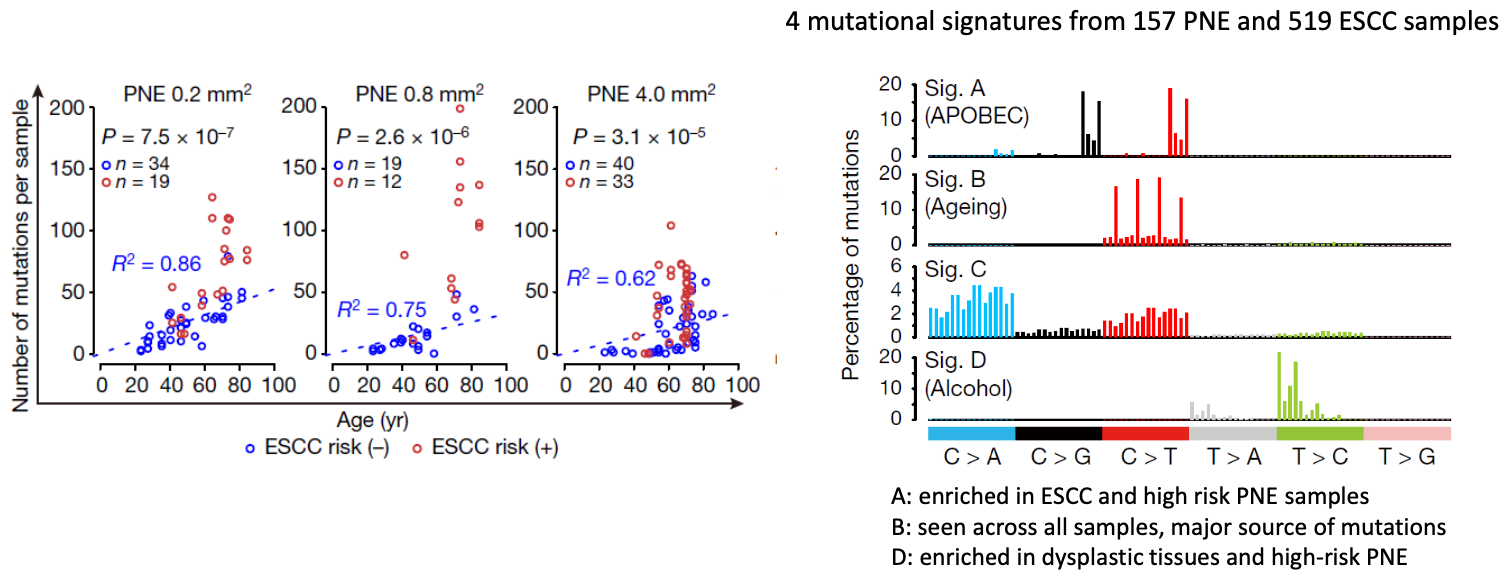
\includegraphics[width=0.5\textwidth]{../_resources/Screen_Shot_2022-11-04_at_10-51-30.png}
\caption{Yokoyama et al., Nature 2019}
\end{figure}

Yokoyama et al., Nature 2019

Normal tissues can accumulate mutations to an extent dependent on lifestyle and age.

Single cell sequencing analysis: the mutation number in colonies from low-risk individuals linearly increases with age with an annual increase of 41.5 mutations per genome per year.

\textbf{\emph{Driver genes}} are mutated in PNE although with different frequencies as compared with
cancer samples and there are substantial differences in the major drivers between PNE and ESCC. Most of the PNE samples from high-risk individuals (62 out of 64, 97\%) contained one or more driver mutations. The positivity of driver mutations was 74\% (69 out of 93) of all samples from low-risk individuals.

\textbf{Spatial distribution and mutational composition of clones within the same biopsy:}

\begin{itemize}
\tightlist
\item
  Young individuals: small number of shared mutations with small MCF. Limited number of driver-mutant clones. During development to early adult life stem cells and their progenies spread giving rise to \textbf{\emph{somatic mosaicism}} more than positive selection.
\item
  Elderly individuals: shared mutations and MCF markedly increase. Driver-mutant clones increase in number and size, a trend which is enhanced with lifestyle ESCC risk. Positive selection may be ongoing.
\end{itemize}

In young individuals we observe a mosaicism of small mutations, while advancing with age we can acquire more mutations which might lead to cell proliferation increase and higher probability of new mutations.

\begin{figure}
\centering
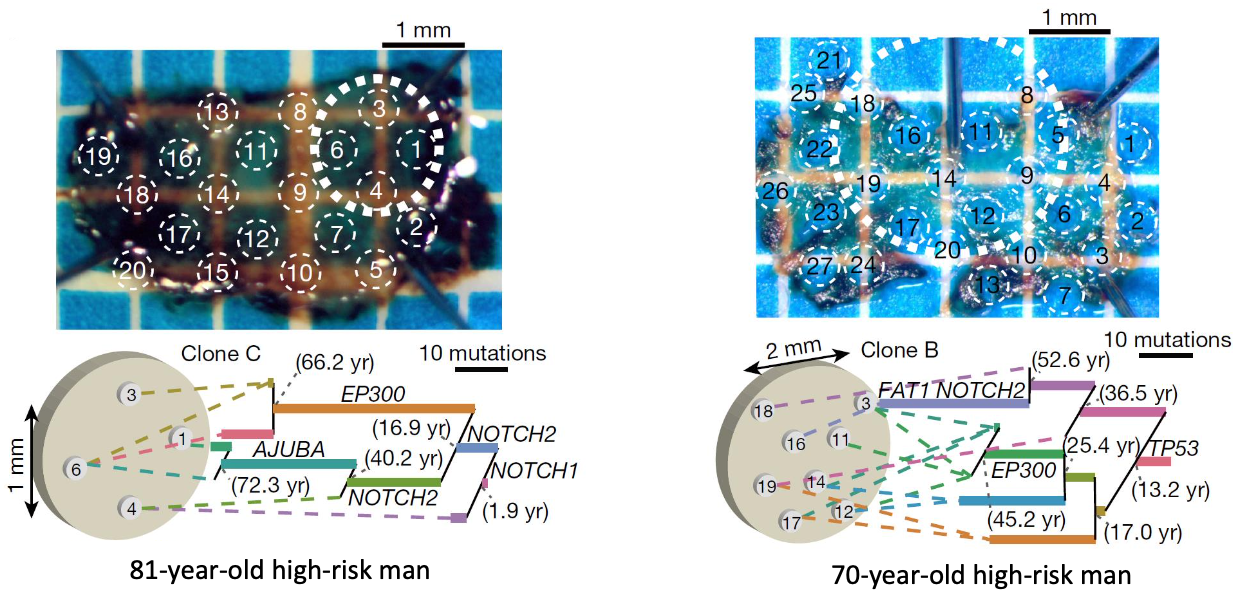
\includegraphics[width=0.5\textwidth]{../_resources/Screen_Shot_2022-11-04_at_10-59-51.png}
\caption{Yokoyama et al., Nature 2019}
\end{figure}

Yokoyama et al., Nature 2019

Some mutations can occur early on in life and they accumulate on specific proliferative pathway they might lead to cancer or not.

80-year-old high-risk man: Divergent clones populating a small epithelial region originated from a single stem cell with a NOTCH1 mutation almost 80 years previously. Positive selection lead to the fixation of 4 driver mutations and subclones formation.
70-year-old high-risk man: Clonal evolution initiated in a stem cell with a TP53 mutation at the age of about 13 years which persisted without evolving to cancer. Meanwhile other driver mutations were acquired.

\textbf{Conclusions}

Mutations inevitably occur in normal cells and accumulate during aging, their frequency depends on lifestyle risks. Such mutations may be positively selected (driver mutations), favoring changes that are beneficial to the individual cells, generating clones. These clones must acquire a number of specific driver mutations to transform generating cancer cells. Normal cells can become cancerous when the `'right'' combination of driver genes has been mutated and/or deregulated. Somatic evolution is not a linear road towards cancer, the clone size, the specific mutations and the tissue context may slow down the tumorigenic process or boost it. Tissues differ substantially in their susceptibility to specific oncogenic events and barriers to tumor formation are tissue specific due to a number of variables, including:

\begin{itemize}
\tightlist
\item
  Tissue-specific oncogenic function of a cancer drivers
\item
  Cell-extrinsic factors such as cell--cell signaling
\item
  The cell of origin and its differentiation status
\end{itemize}

With age, the spreading of mutant clones within tissues may progressively compromise the tissue contributing to aging, cancer and other diseases.

The same pattern was observed in colorectal tissue and especially skin, which has a high burden of somatic mutations.

Standard chemotherapy relies on targeting proliferating cells with alkylating agents. We can also apply precision therapy to certain oncogenes, but this approach should take into account that multiple mutations are present. Over the years, it was observed that if the expression of a target oncogene is repressed, we observe growth inhibition and tumor regression.

Cancer cells can become addicted to the expression of specific oncogenes

Important bias: we are inducing tumorigenesis by inducing overexpression of a single gene, which is not what happens physiologically. However, we know have in clinics drugs targeting different proteins and able to induce tumor regression. One of the first compounds developed was Imatinib, meant to target a kinase fused in CML. Roughly 53 out of 54 patients were cured in phase I clinical trial. All the targets hit by target therapy drugs are enzymes, most of them kinases.

Cancer cells tend to lose cellular functions which are not essential to cell viability or do not increase cellular fitness. This is due to the \emph{genetic drift} determined by the mutational burden, epigenetic modifications, and tumor microenvironment. The silencing of redundant functions and pathways can render cancer cells more susceptible to perturbations. If we hit a particular pathway in a cell, we can impair a function which was previously regulated by multiple pathways $\rightarrow$ synthetic lethality.

If the domain changes e.g.~accumulation of mutations on oncogene, cancer cells can develop resistance to target therapies. The same happens with new mutations on alternative pathways.

\begin{figure}
\centering
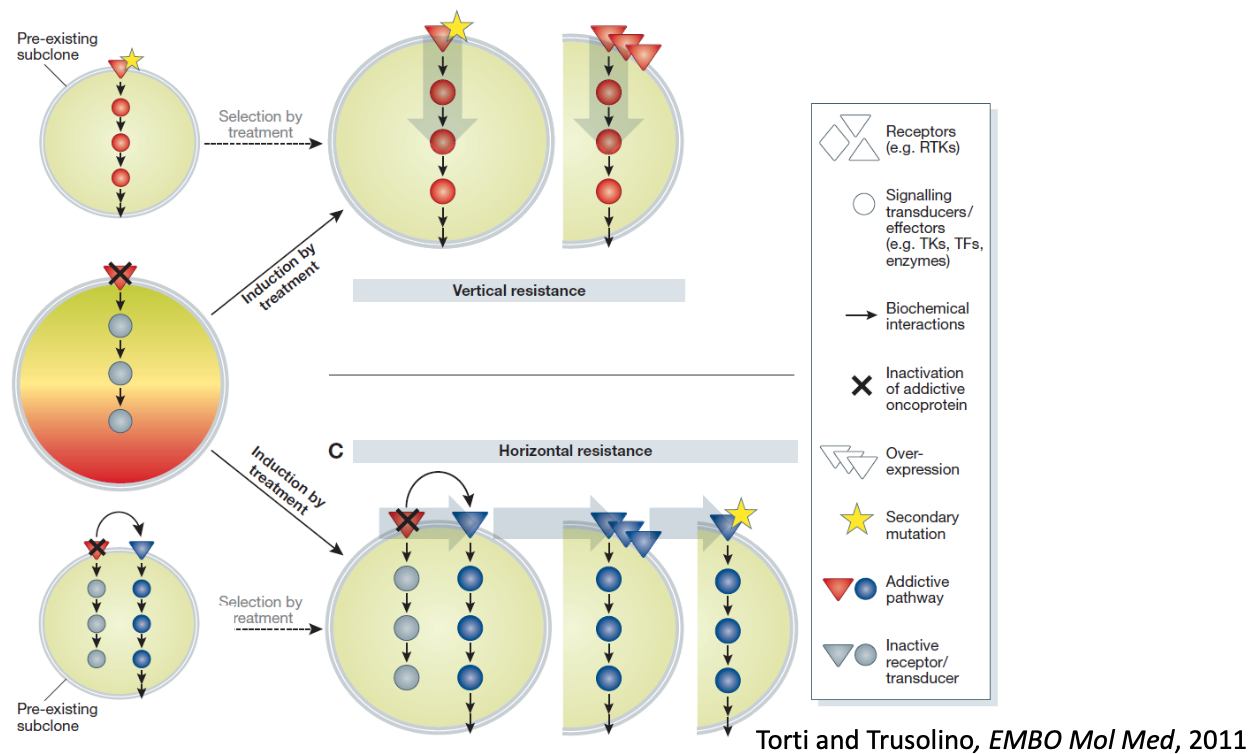
\includegraphics[width=0.5\textwidth]{../_resources/Screen_Shot_2022-11-04_at_11-25-54.png}
\caption{Screen Shot 2022-11-04 at 11.25.54.png}
\end{figure}

 Targeted therapeutics generally lead to resistance

Transcriptional regulators are essential effectors of the transcriptional program imposed by oncogenic drivers, also called transcriptional drivers.

RTK growth factor, frequently hit by mutations in cancer. Resistance can arouse through the persistence of downstream pathway or parallel signaling transduction. This occurs as pathways converge to the same effectors, which are either co-factors regulating transcription or transcription factors. E.g. MYC or beta-catenin, which are also called \emph{transcriptional drivers}.

Example: MYC inhibition eradicates K-RAS (driver oncogene) driven lung cancers in mice.

The consequences of oncogene inactivation for the reversal of tumorigenesis depend on the type of tumor and the genetic context. E.g. if we remove MYC from MYC driven lymphoma, we observe apoptosis of lymphoma cells. In hepatocellular carcinoma, the re-expression of MYC leads to restoring cancer. Cancer cells can escape dependence on oncogenes by acquiring other genetic events.

\hypertarget{key-points}{%
\subsubsection{Key points}\label{key-points}}

Cancer is caused primarily by genetic mutations and is initiated and maintained by recurrent driver mutations. Cancer cells genome undergoes a constant genetic drift. Transcription deregulation is a hallmark of cancer, as cancer cells inevitably undergo transcription rewiring. Dysregulated transcriptional programs fuel tumorigenesis. Cancers can remain addicted to the oncogenes that have driven tumorigenesis and/or to the transcriptional drivers (definitive cancer drivers). Dysregulated transcription also creates transcriptional dependencies which are not typically identified by cancer genome sequencing. \textbf{Transcriptional addiction} in cancer can be harnessed for therapeutic intervention.

Resistance to targeted therapy can occur by activating \emph{alternative signaling molecules} and pathways converging on the same transcriptional regulators or by \emph{acquiring mutations} on the targeted gene.

Transcriptional regulators act as effectors of the oncogenic drivers. Cancer cells can become as `'addicted'' to these effectors as they are to the oncogenic drivers.

The complexity of TFs networks renders resistance mechanisms difficult to be developed.

Transcription factors interact in complex networks, also involving other transcription regulators. It is unlikely that any TF, or non-TFs transcriptional regulators such as CBP-p300, BRD4, can be completely replaced by another. It is more difficult to bypass this particular targeting.

\begin{figure}
\centering
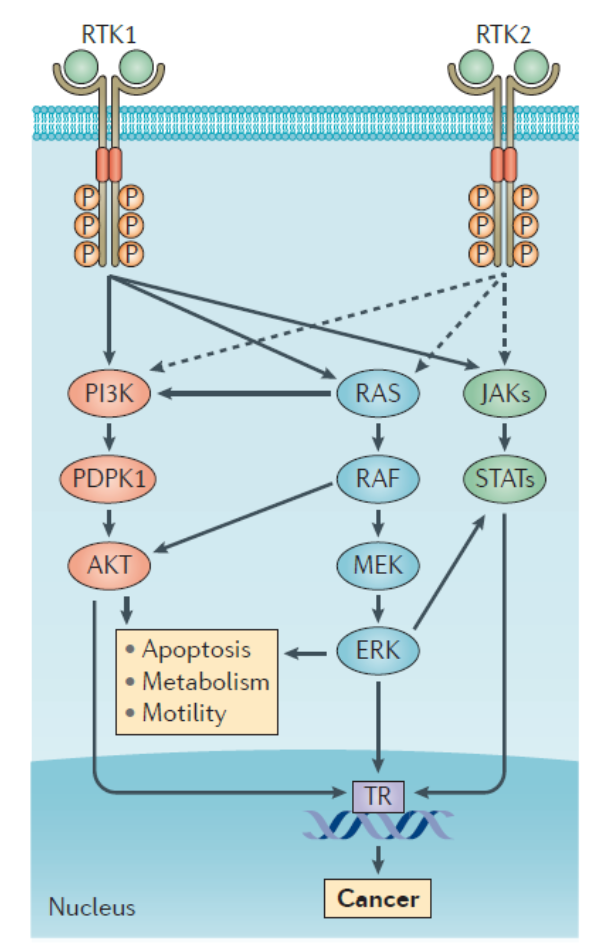
\includegraphics[width=0.5\textwidth]{../_resources/Screen_Shot_2022-11-04_at_11-51-12.png}
\caption{Gonda and Ramsay, \emph{Nature Review Mol Cell Biology}, 2015}
\end{figure}

Gonda and Ramsay, \emph{Nature Review Mol Cell Biology}, 2015

Targeting transcription regulators will have a lower likelihood of emergence of resistance than targeting intracellular signaling pathways, also because multiple pathways can converge on the same transcription regulator. Inhibiting a specific transcriptional program may impact more than one oncogenic signal. The main issue is to identify transcriptional drivers, which might not be affected by mutations; it is required to perform wet lab experiments. Furthermore, target mutations can still emerge as resistance mechanism.

\hypertarget{target-transcription-in-cancer}{%
\subsection{Target transcription in cancer}\label{target-transcription-in-cancer}}

There exist numerous ways to target transcription in cancer:

\begin{itemize}
\tightlist
\item
  interaction with co-factor
\item
  interaction with ligand $\rightarrow$ most effective mechanism, clinical trials
\item
  PTM
\item
  TF-TF interaction
\item
  impairing recruitment to responsive elements
\end{itemize}

The mechanism of action can be PROTAC or monomeric degradation: they bind their own target and promote degradation. The \textbf{monomeric degrader} can alter 3D structure to make accessible to proteosomal degradation. \textbf{PROTAC} has a domain for E3 ligase, which leads to the recruitment of protease. In principle these molecules can interact with any region of the protein e.g.~epitope, AA sequence (not necessarily domain). Once the protein is degraded, the molecule is still around and can be recycled to degrade other proteins (1:1 stoichiometry is not required).

\begin{figure}
\centering
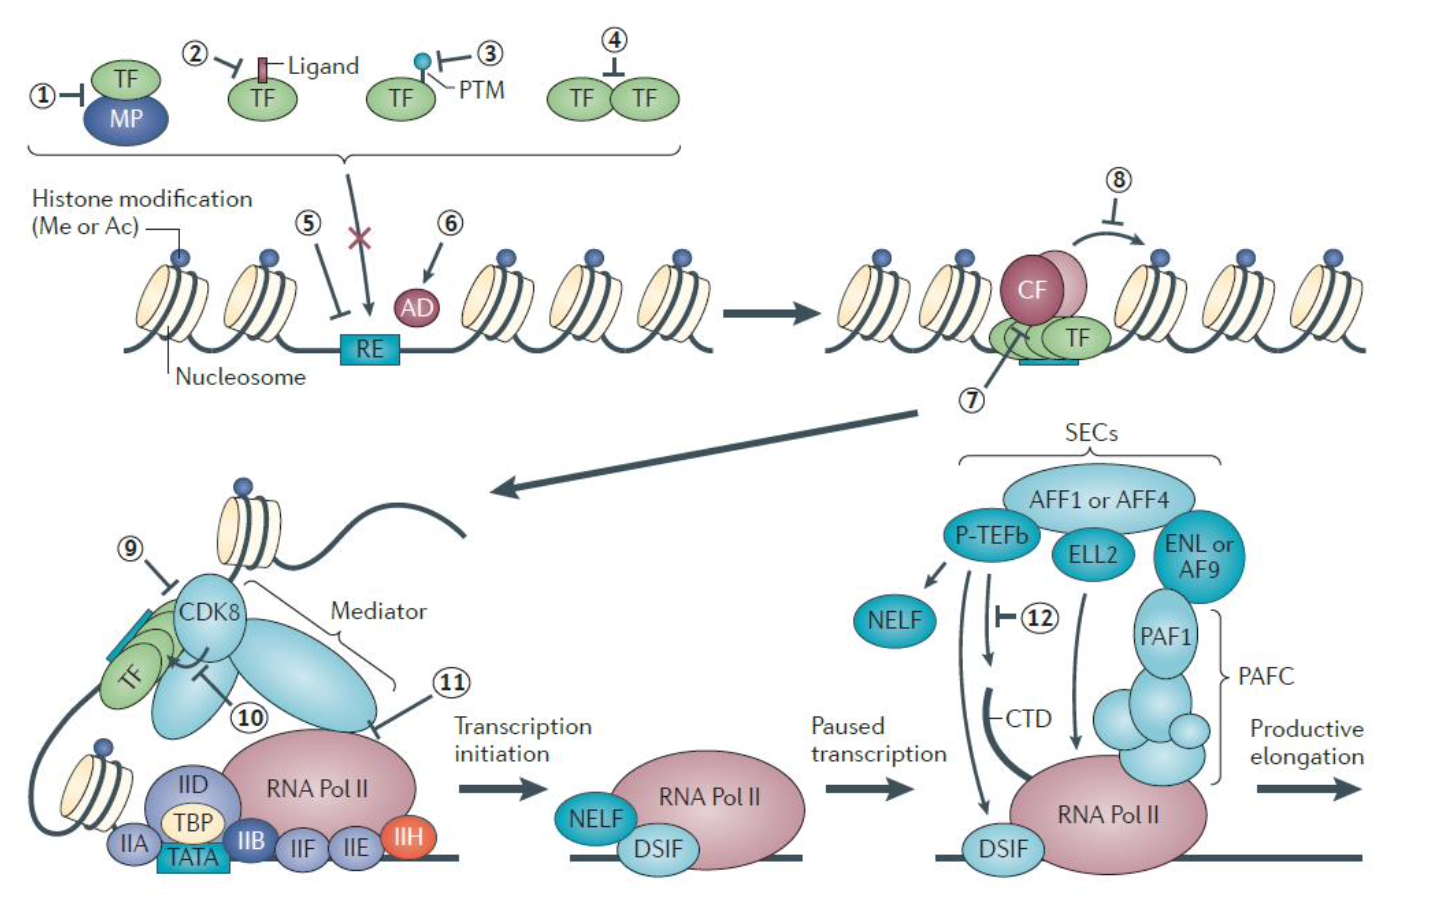
\includegraphics[width=0.5\textwidth]{../_resources/Screen_Shot_2022-11-04_at_11-55-34.png}
\caption{Bywater \emph{et al., Nature Review Cancer-} 2013}
\end{figure}

Bywater \emph{et al., Nature Review Cancer-} 2013

The Mediator and other complexes are controlled by kinases, so we can foster their inhibition.

THZ1 interacts with the ATP binding pocket of CDK-7, covalent bond with Cys321. In the study the THZ1-R,R was used as a control, as it should not achieve Cys binding.

By pulling down THZ1, we can visualize CDK7 activity: by increasing the amount of THZ1, the competition with bio-THZ1 is overcome and CDK7 expression is inhibited. RNAPII phosphorylation is impaired in vitro with high amounts of THZ1. If the experiment is performed with mutated C312S, phosphorylation of Pol II is not inhibited anymore.

Washout experiment: treat compound, wash and let cells grow without the compound. In this case CDK7 inhibition persists, since it is irreversible thanks to covalent binding.

THZ1 treatment shows broad antiproliferative activity in cancer cell lines by modulation of transcription.

High throughput screening of cell lines in micro plates to test cell proliferation shows that T-ALL cells are particularly sensitive to small perturbations in transcription and CDK7 kinase function. Instead BJ fibroblasts and RPE-1 were not affected.

Bioluminescent xenografted mouse model confirmed efficacy of THZ1 in blocking tumorigenesis of the human T-ALL cell-line KOPTK1. No toxicity of the compound was observed in mice. High doses of THZ1 were required to impair proliferation of non transformed cells.

\emph{Why do cancer cells and in particular T-ALL cells are more sensitive to CDK7 inhibition than non cancer cells?} By applying 250 nM of THZ1 we observe the reduction of transcription of all genes. If we lower the concentration at 50 nM, only a subset of genes will be impacted e.g.~TAL1, GATA3, RUNx1 $\rightarrow$ super enhancer region, these factors autoregulate their own gene expression while simultaneously regulating many other genes.

 RUNX1 forms a core regulatory circuitry with TAL1 and GATA3 transcription factors that have prominent roles in leukaemia biology

\textbf{Takehome message:}

Targeting transcription is a promising anticancer approach which can be achieved by CDK7 inhibition. Transcription rewiring of cancer cells can be triggered by acquisition of super-enhancers driving oncogene expression and tumorigenesis. Super-enhancer driven oncogenes lead to transcription addiction generating transcriptional dependencies which can be used for therapeutic intervention. Cancer cells require continuous active transcription which renders them more sensitive to transcription targeting therapeutics. In particular oncogenic drivers like MYC and RUNX1 have short mRNA and protein half-lives and depends on continuous transcription. Genomic sequences may not suffice to identify driver oncogenes and cancer vulnerabilities.

\hypertarget{transcriptional-control-in-cancer}{%
\section{15- Transcriptional Control in Cancer}\label{transcriptional-control-in-cancer}}

\hypertarget{brd4}{%
\section{BRD4}\label{brd4}}

BRD4 is a member of the Bromodomain and Extraterminal (BET) family along
with BRD2, BRD3 and BRDT. It is a histone acetyltransferase that evicts nucleosomes from chromatin. In particular, BET inhibitors impair super-enhancer driven oncogene expression.


\begin{figure}
\centering
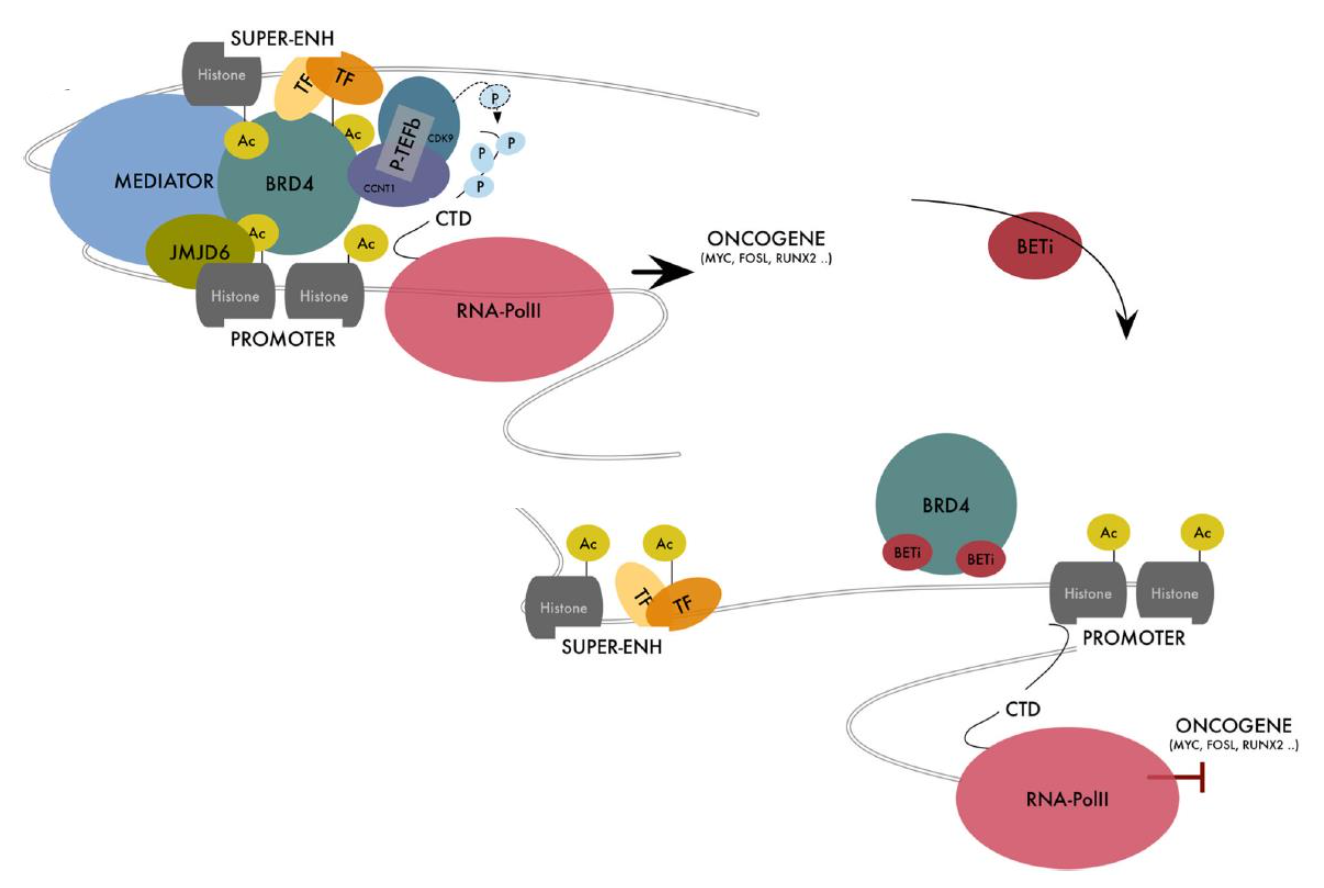
\includegraphics[width=0.5\textwidth]{../_resources/Screen_Shot_2022-11-13_at_19-35-28.png}
\caption{Screen Shot 2022-11-13 at 19-35-28.png}
\end{figure}

\hypertarget{selective-inhibition-of-tumor-oncogenes-by-disruption-of-super-enhancers}{%
\subsubsection{Selective inhibition of Tumor Oncogenes by Disruption of Super-Enhancers}\label{selective-inhibition-of-tumor-oncogenes-by-disruption-of-super-enhancers}}

Super-enhancers associated genes were expressed at higher levels than enhancer-driven genes and specifically in mieloma cell line. The majority of super enhancer associated genes were previously shown to be involved in mieloma tumorigenesis e.g.~MYC, CCND2. Treatment of MM1 cells with Brd4 inhibitor JQ1 resulted in reduced levels of BRD4 at enhancers and promoters.

JQ1 treatment lead to more pronounced reduction of BRD4 enrichment at super- enhancers showing almost complete loss of BRD4; in particular, super-enhancers are more sensitive to BRD4 inhibition than regular enhancers. MYC is among the most rapidly depleted genes upon BRD4 inhibition.

Genes associated with super-enhancers showed greater decrease in RNApol II at gene body than the ones associated with enhancers.

\begin{itemize}
\tightlist
\item
  Cancer cells can acquire super-enhancers (SE) as mechanism to drive oncogene expression
\item
  SE are characterized by disproportionately high levels of BRD4 and Mediator, interacting with each other and with multiple cofactors
\item
  SE are highly reliant on cooperatively interacting factors and lose activity more rapidly (than enhancers) when the levels of SE-bound factors are reduced
\item
  BRD4 inhibition leads to preferential disruption of SE driving critical oncogenes in cancer cells
\end{itemize}

The molecular details underlining cancer cells addiction to BRD4 are being unveiled.

\hypertarget{yaptaz}{%
\section{YAP/TAZ}\label{yaptaz}}

The transcriptional coactivators YAP (Yes-associated protein)/ TAZ (transcriptional coactivator with PDZ-binding motif) and their interactors.

\begin{figure}
\centering
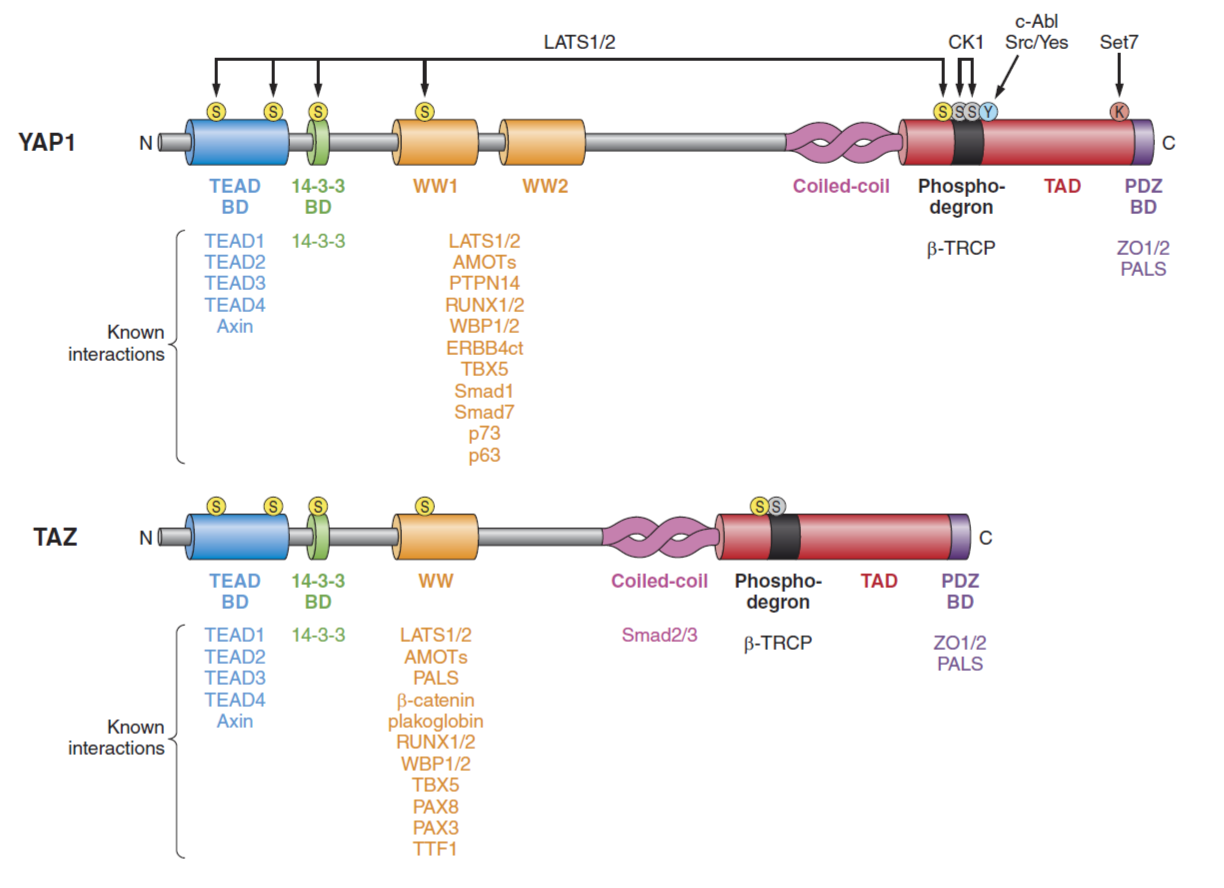
\includegraphics[width=0.5\textwidth]{../_resources/Screen_Shot_2022-11-13_at_19-40-17.png}
\caption{Screen Shot 2022-11-13 at 19-40-17.png}
\end{figure}

The \textbf{HIPPO signalling} regulates YAP/TAZ and epithelial architecture and cell polarity are inhibitors of YAP/TAZ $\rightarrow$ EMT triggers inactivation of the Hippo cascade and YAP/TAZ activation.

\begin{figure}
\centering
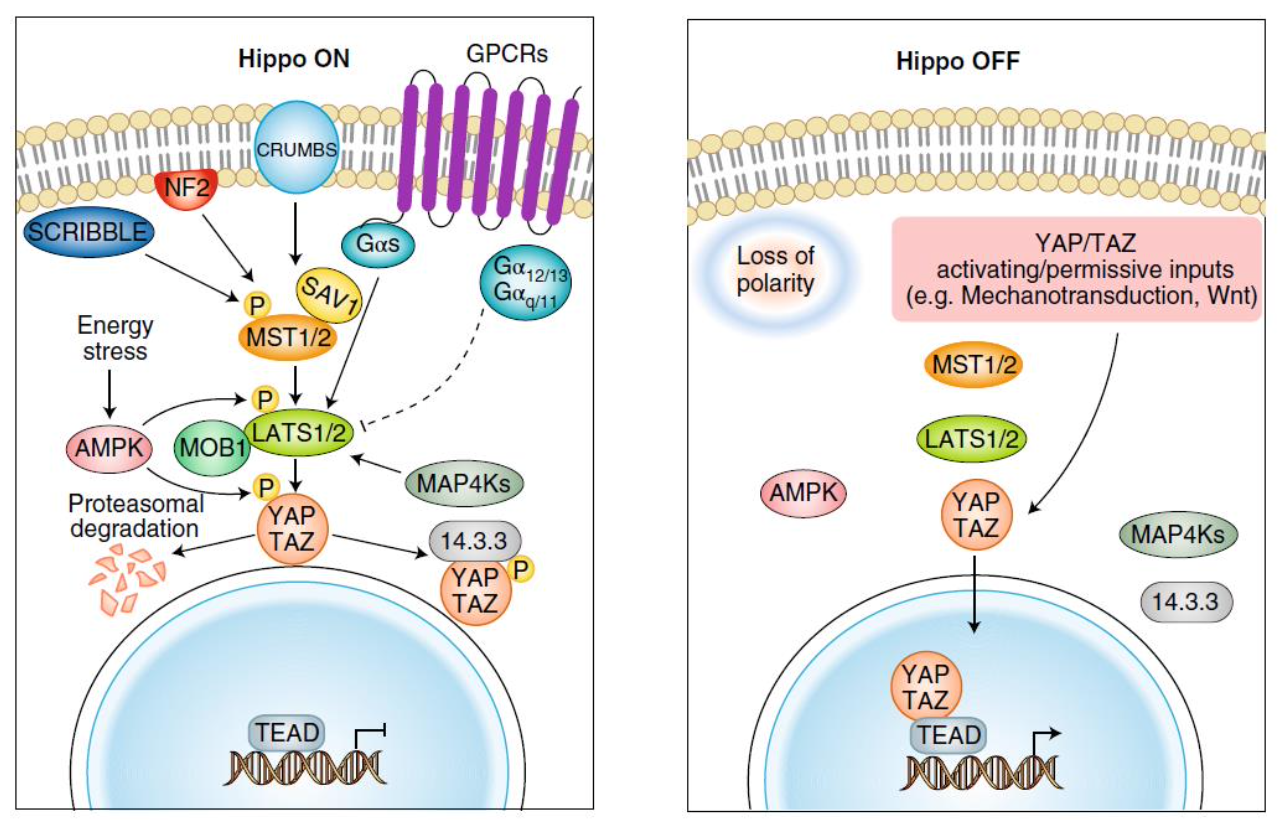
\includegraphics[width=0.5\textwidth]{../_resources/Screen_Shot_2022-11-13_at_19-41-35.png}
\caption{Screen Shot 2022-11-13 at 19-41-35.png}
\end{figure}

Mechanical signals are ubiquitous, targeting every cell in every tissue. Mechanotransduction converge on YAP/TAZ in multiple cellular contexts.

YAP and TAZ are nuclear effectors of mechanical signals exerted by ECM and cell shape:

\begin{figure}
\centering
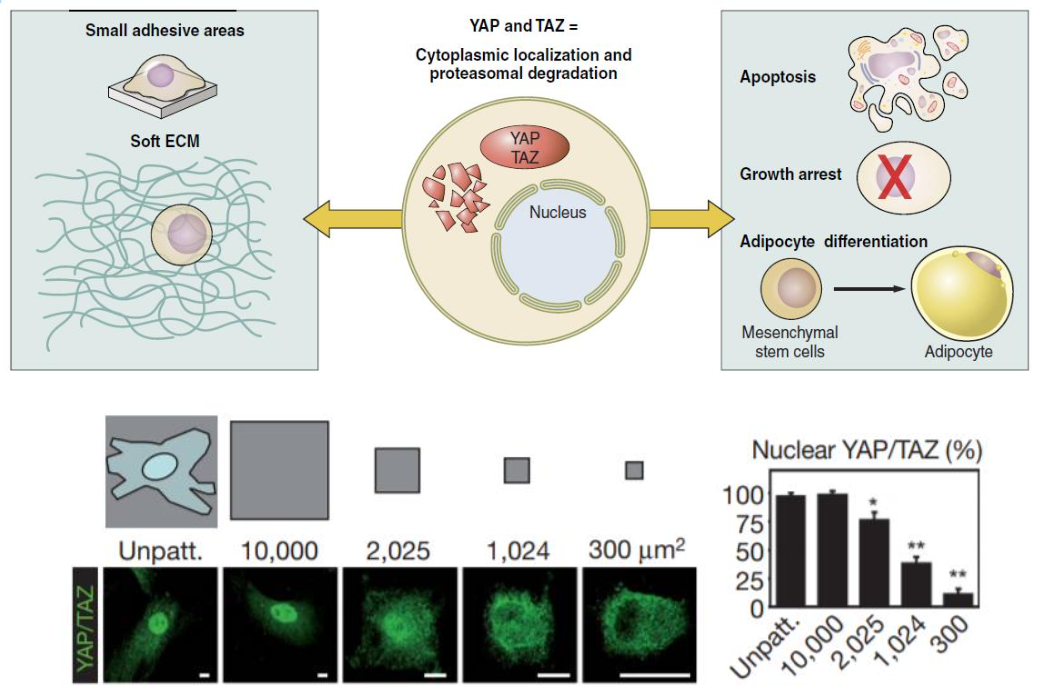
\includegraphics[width=0.5\textwidth]{../_resources/Screen_Shot_2022-11-13_at_19-43-07.png}
\caption{Dupont et al., Nature 2011}
\end{figure}

Dupont et al., Nature 2011

The process of tumorigenesis is accompanied by collagen crosslinking, ECM stiffening, and increased focal adhesions. YAP/TAZ activity is controlled by cell shape and polarity through the cytoscheletal structure which also senses the topology and the rigidity of the extracellular matrix.

Cells probe the physical features of the microenvironment through integrins and adesive proteins responding to extracellular forces by adjusting their tensional state through the cytoscheleton activity. Physical and mechanical cues transmitted by the extracellular environment (i.e.: stiffness of the ECM) reach the nucleus at least in part by YAP/TAZ activation.

YAP/TAZ interact with the TEAD transcription factors to regulate gene expression.

\hypertarget{tead}{%
\section{TEAD}\label{tead}}

\begin{figure}
\centering
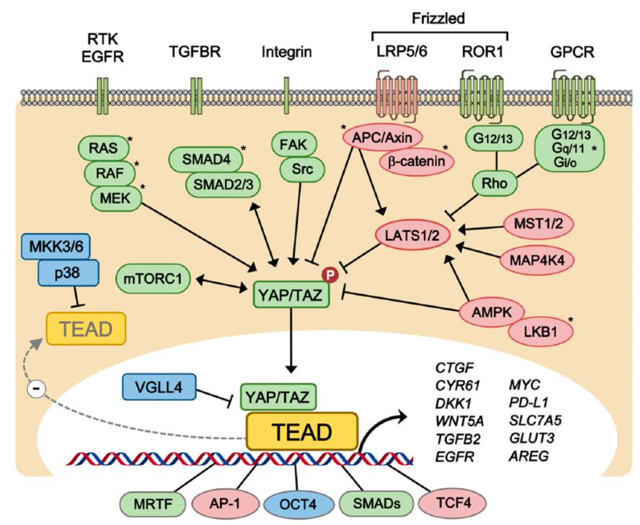
\includegraphics[width=0.5\textwidth]{../_resources/Screen_Shot_2022-11-13_at_19-48-01.png}
\caption{Screen Shot 2022-11-13 at 19-48-01.png}
\end{figure}

TEAD is regulated by Hippo, Wnt, TGF-beta and EGFR pathway and is responsible for controlling drug resistance, metastasis, EMT and cancer stem cells. TEAD-driven transcriptional targets include well-established genes that are involved in cell growth, proliferation, and tissue homeostasis. YAP/TAZ drive several key attributes of cancer cells.

\hypertarget{yaptaztead}{%
\subsection{YAP/TAZ/TEAD}\label{yaptaztead}}

Mapping YAP/TAZ/TEAD associations with chromatin in breast cancer cells reveals that these regulators associate with active enhancers. Hi-C analyses predict about 3000 genes regulated by YAP/TAZ/TEAD. 3C analyses confirmed YAP/TAZ/TEAD binding to MYC and TOP2A enhancers.

YAP/TAZ are required for activation of MYC and TOP2A enhancers.

YAP/TAZ-depleted cells stop proliferating and accumulate in G1.

TEAD depletion phenocopies YAP/TAZ depletion $\rightarrow$ TEAD is determinant for YAP/TAZ induced proliferation. Most YAP/TAZ motifs contained both TEAD and AP-1 motif.

Requirement of AP-1 for YAP/TAZ/TEAD induced transcription program tumorigenesis.

YAP/TAZ interact with the TEAD transcription factors to regulate gene expression. AP-1 enhances YAP/TAZ/TEAD transcription program and tumorigenesis

BRD4 inhibition impacts the YAP/TAZ transcriptional program in the MDA-MB-231 breast cancer cell line $\rightarrow$ \textbf{Brd4 is required for YAP/TAZ-mediated transcriptional regulation}. In addition YAP/TAZ are required for BRD4 recruitment to chromatin.

Conclusions:

\begin{itemize}
\tightlist
\item
  YAP/TAZ and BRD4 associate physically and functionally in breast cancer cell lines
\item
  YAP/TAZ-BRD4 complex confers a transcriptional advantage to a broad YAP/TAZ targets the expression of these genes can be targeted by BET inhibitors
\item
  Super-enhancers consist of YAP/TAZ-occupied enhancers showing strong enrichment of BRD4, high expression levels of regulated genes and higher sensitivity to BET inhibitors than average
\item
  Oncogenic effect of BRD4 in association to YAP/TAZ offers a new perspective:
  to stratify patients which are more likely to benefit from BET inhibitors, alone or in combination with other drugs
\item
  Development of new therapeutic approach around YAP/TAZ-BET interaction surfaces
\end{itemize}

$\rightarrow$ YAP/TAZ represent ideal candidates to mediate cancer-specific transcriptional addictions
and potential drug targets


\hypertarget{transcriptional-control-in-cancer}{%
\section{17- Transcriptional Control in Cancer}\label{transcriptional-control-in-cancer}}

Recap

{[}\ldots{]} copy from slides

The inhibition of BRD4 could represent an important mechanism to target.

If we analyze tumorigenic mechanisms in vivo and in vitro we will observe different results: processes dictated by the microenvironment will significantly impact on the tumorigenic potential of cancer cells.

Binary pan-cancer: YAP/TAZ are upregulated oncogenes. Cancers that do not express YAP/TAZ can silence its expression, as it will lead to cell death and differentiation. The effect of YAP/TAZ all depends on the transcriptional program. It is possible to impair YAP/TAZ through targeted therapies e.g.~Tyr kinase inhibitors or Ser/Thr kinase inhibitors; however we must be careful, as resistance can arise. When the transcriptional program is inhibited, tumor suppression is observed. In the case of YAPoff cancers we observe the expression of MYC, which could be targeted. If we manage to re-express YAP/TAZ, they will bind to TEAD and bHLH activating genes promoting adhesion and cell differentiation, always resulting in tumor suppression.

\begin{figure}
\centering
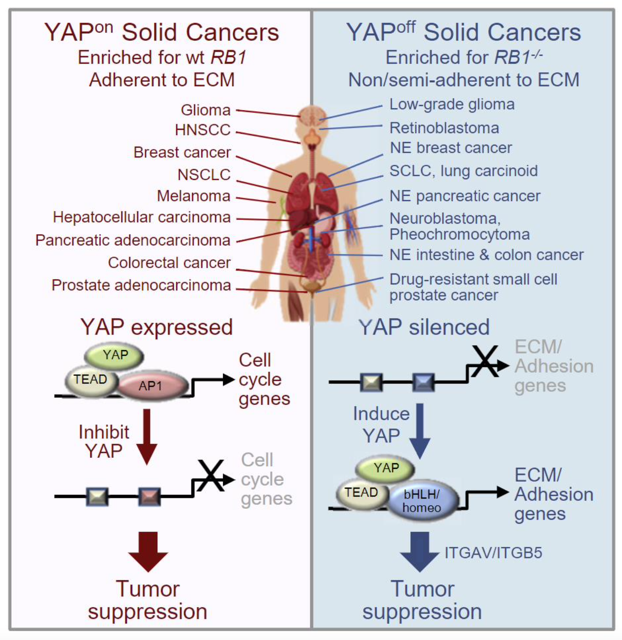
\includegraphics[width=0.5\textwidth]{../_resources/Screen_Shot_2022-11-18_at_11-11-12.png}
\caption{Screen Shot 2022-11-18 at 11-11-12.png}
\end{figure}

\hypertarget{nuclear-receptors}{%
\section{Nuclear receptors}\label{nuclear-receptors}}

Nuclear receptors are transcription factors which mediate transcription regulation upon receptor-specific ligand binding. Usually NR are found bound to DNA in the nucleus or to other proteins in the cytoplasm. In most of the cases they are hetero or homodimers. Nuclear receptors share a common architecture - very conserved modular structure composed by 2 transactivator domains, DNA binding domain and C terminus ligand binding domain (11 helices forming a pocket, 12th helix outside acting as a pocket closure) - and functional behavior. NR are involved in many processes and in different forms of cancer e.g.~estrogen receptor alpha ((ER$\alpha$)).

ER$\alpha$ is associated with proliferation and development and cells for the formation of tissues and organs in women. ER$\beta$ has the opposite function, it is repressing proliferation. ER$\alpha$ is expressed in mammary glands and uterus., ER$\beta$ colon or immune system cells. It is still unclear how the two behave so differently, probably specific TF interaction.

\hypertarget{estrogen-receptor-alpha}{%
\subsection{\texorpdfstring{Estrogen receptor \(\alpha\)}{Estrogen receptor \textbackslash alpha}}\label{estrogen-receptor-alpha}}

Estradiol induces dimerization of ER and binding of the dimer to ER response elements (EREs). ER$\alpha$ binds to HSPs and when estradiol is met we observe the conformational change leading to ERE binding. For achieving a complete activation of the NR, PTMs are required e.g.~Cdk7 targets S118 for phosphorylation.

The main antagonists of ER are known as \textbf{SERM} and \textbf{SERD}. The first target therapy for ER, \emph{Tamoxifen}, was developed in the late 60s. Tamoxifen belongs to SERM, modulator interacting with ER, impairing the ability to interact with the binding site. Once ER binds it cannot recruit co-regulators, its transcriptional action is shut down. Short term Tamoxifen treatment does not show high survival rates, but longer times expose patients to side effects e.g.~acts as agonist for ER in endometrial cells. Other drugs from SERM family act similarly e.g.~Raloxifene and Bazedoxifene. In addition to SERM, we have ER degraders from SERD family $\rightarrow$ through degradation PTMs e.g.~sumoylation. Fulvestrant is a steroid derivative molecule (quite different from Tamoxifen), not water soluble so needs to be injected in muscles.

\begin{figure}
\centering
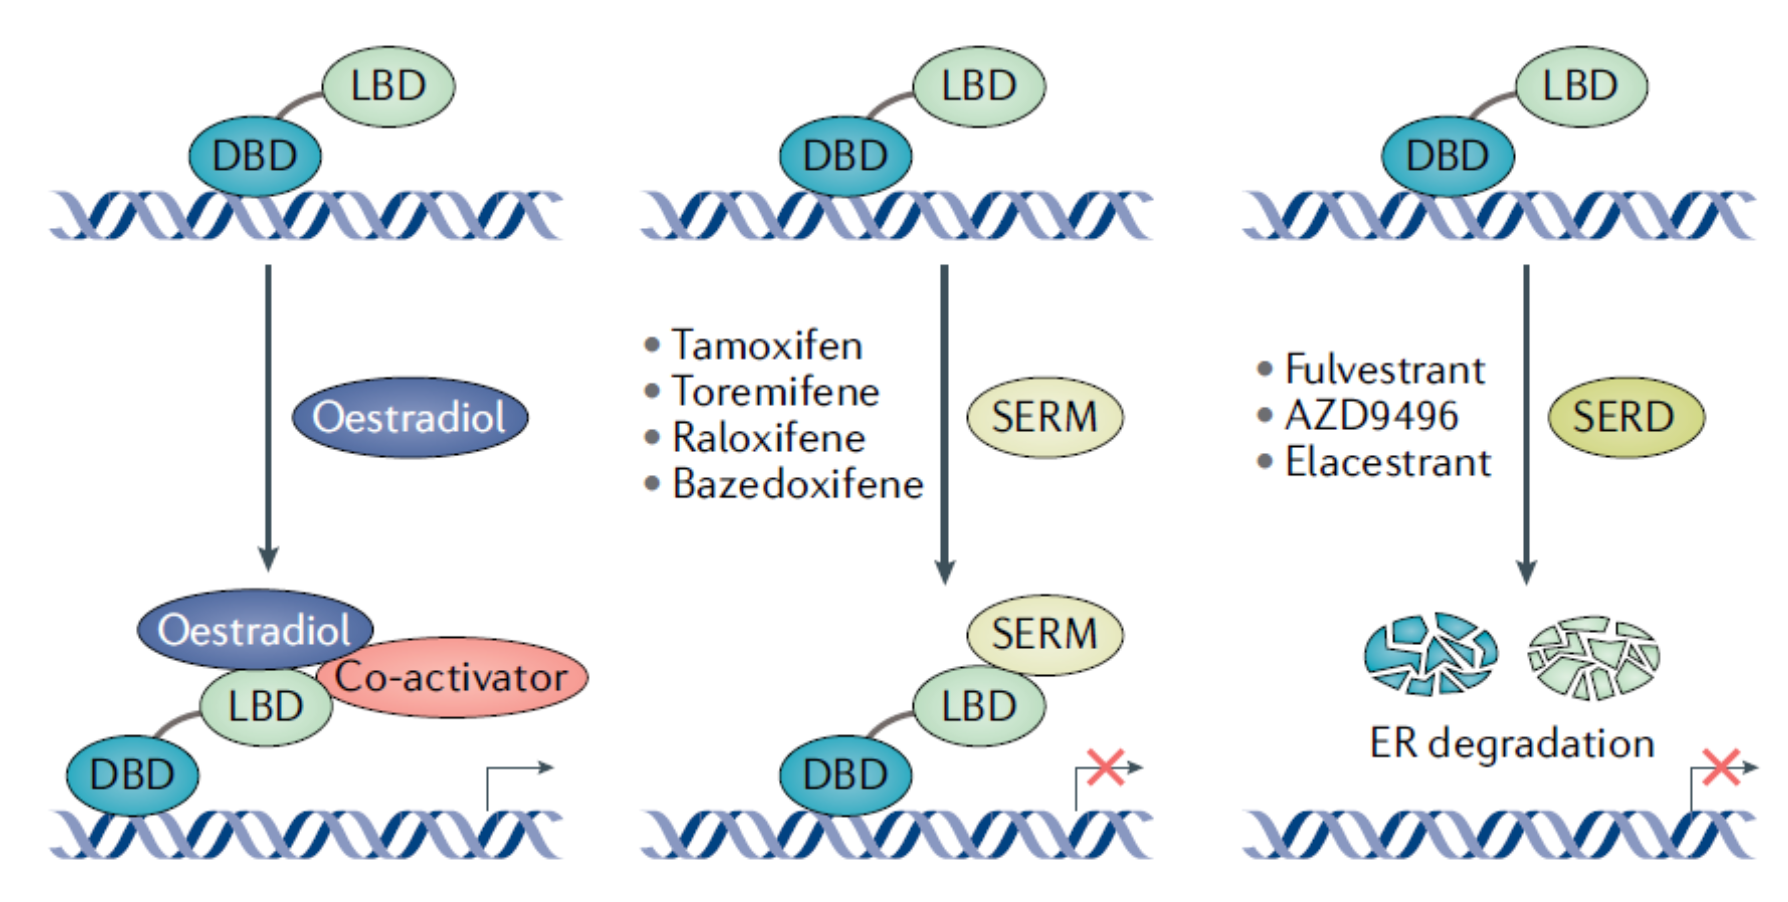
\includegraphics[width=0.5\textwidth]{../_resources/Screen_Shot_2022-11-18_at_11-06-54.png}
\caption{Screen Shot 2022-11-18 at 11-06-54.png}
\end{figure}

The two major strategies for therapeutic targeting of hormonal signaling in breast cancer are \emph{direct antagonism} of the ER and \emph{estrogen deprivation}. Aromatase inhibitors can avoid estradiol production in order to deactivate ER activation.

\begin{figure}
\centering
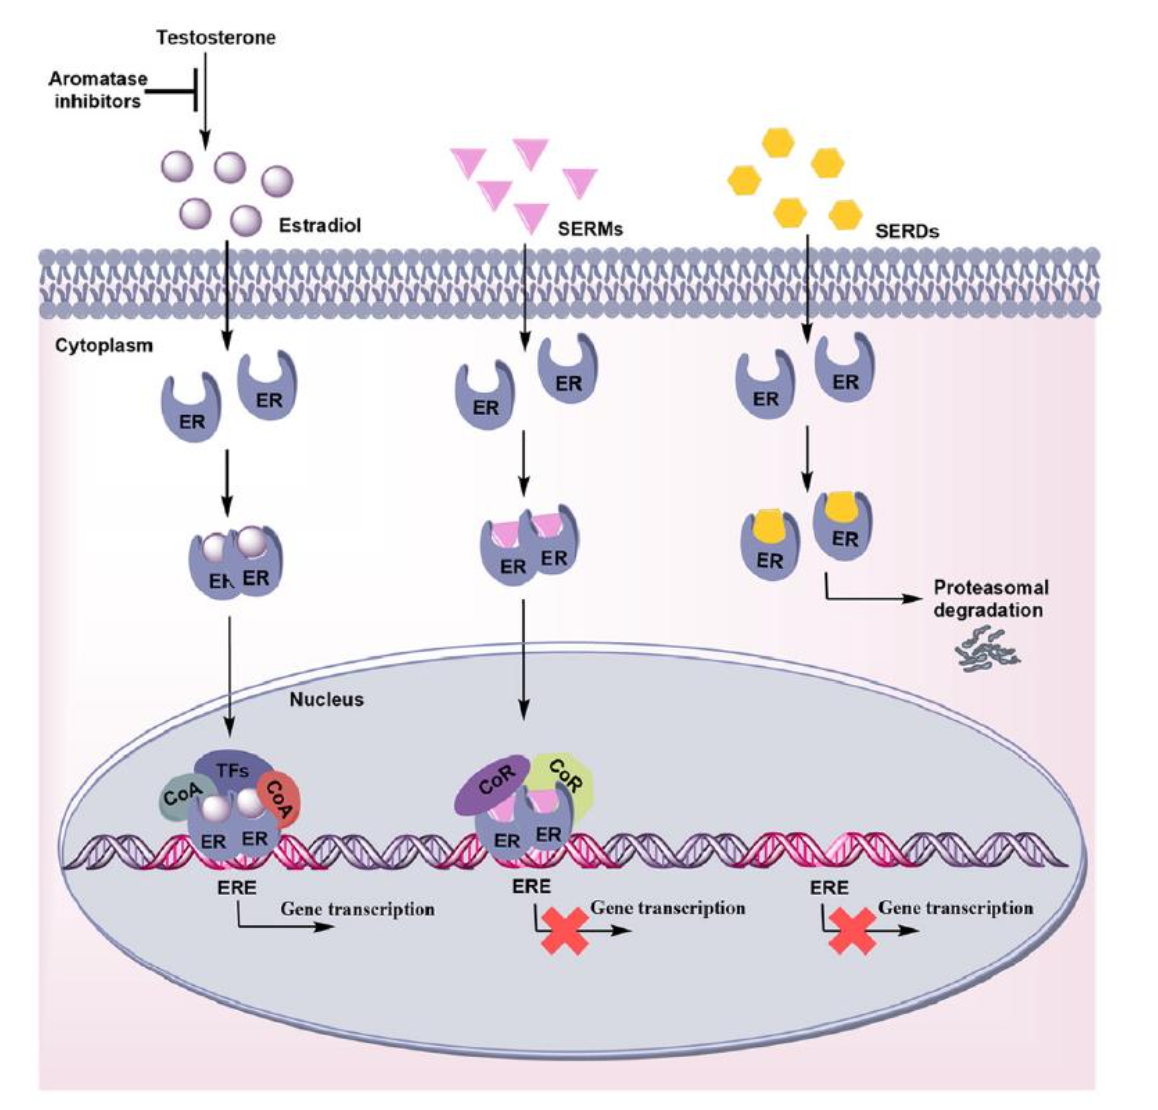
\includegraphics[width=0.5\textwidth]{../_resources/Screen_Shot_2022-11-18_at_11-14-09.png}
\caption{Screen Shot 2022-11-18 at 11-14-09.png}
\end{figure}


\subsection{ER$\alpha$) in breast cancer}

\begin{itemize}
\tightlist
\item
  Nearly 75\% of breast cancers are driven by ER$\alpha$-mediated transcriptional activity
\item
  Estrogen deprivation and direct antagonism of ER represent the two major strategies for therapeutic targeting of ER+ breast cancers
\item
  More than 20\% of patients develop resistance to anti-estrogens and relapse with metastatic disease
\end{itemize}

\hypertarget{mechanisms-provoking-breast-cancer-drug-resistance}{%
\subsubsection{Mechanisms provoking breast cancer drug resistance}\label{mechanisms-provoking-breast-cancer-drug-resistance}}

Clinical sequencing of 11 metastatic ER-positive breast cancer cases before and after therapy showed that \textbf{ESR1 mutations} were not present at an earlier stage, indicating that they were acquired after endocrine therapy. Tumors had survived estrogen targeting or deprivation treatments by acquiring ESR1 mutations.

ESR1 alterations are focused on H12 of the LBD. Analyses of 390 ER-positive breast cancers (primary tumors, before hormonal treatment) from the TCGA revealed no LBD-disrupting mutations of ESR1.

ESR1 with acquired mutations encode constitutively active proteins functioning in the absence of ligand $\rightarrow$ resistance mechanism. The mutated ESR1 variants are active in the absence of estrogen and continue to be responsive to direct ER antagonists. These mutations might not have been arisen under selective pressure of anti-estrogen treatment but rather in the context of an estrogen deprivation setting, such as treatment with aromatase inhibitors and/or oophorectomy. 67.4\% of the ESR1-mutant metastatic patients had prior exposure to an aromatase inhibitors.

The presence of a somatic mutation in the LBD of ESR1 does not necessarily imply constitutive activity. The most frequent mutation is D538G. Most mutations were activating ER in the absence of estradiol. ER mutants show increased S118 and S167 steady state phosphorylation.

Fulvestrant (ICI) was able to inhibit the activity of all of the mutants which however showed significant differences in sensitivity to the drug. Y537S mutants displayed 70-fold higher IC99 than WT ER, while E380Q and S463P showed 2-fold higher IC99. Fulvestrant fully inhibited the growth of the WT-, E380Q-, and S463P expressing tumors while nearly completely inhibiting the growth of D538G tumors. The Y537S-expressing tumors, however, continued to grow in the presence of fulvestrant, albeit more slowly than in untreated controls, AZD9496 was able to completely inhibit their growth.

These findings are consistent with results from a subsequent clinical trial identifying the ER$\alpha$ Y537S as an acquired mutation promoting resistance to fulvestrant treatment.
Patients previously progressing on endocrine therapy were enrolled for either palbociclib plus fulvestrant or placebo plus fulvestrant treatment, demonstrating an improvement in median PFS from 4.6 to 11.2 months with the addition of palbociclib to fulvestrant. Acquisition of new PIK3CA and ESR1 mutations, in particular the ESR1 Y537S mutation, in both treatment arms implicates these changes in the development of parallel mechanisms of resistance and suggest potential new avenues for treatment.

\hypertarget{summary}{%
\subsubsection{Summary}\label{summary}}

\begin{itemize}
\tightlist
\item
  \emph{ESR1 gene mutations} are found in about \textbf{14\% of breast cancer metastasis}
\item
  Most ER mutations promote an activated conformation in the absence of ligand which remains
  permissive for ligand binding, thus a direct antagonism may be a strategy for these mutants
\item
  Mutations behave differently in terms of ER activity and sensitivity to drugs
\item
  Mutated-ER proteins can be inhibited by \emph{fulvestrant} and \emph{AZD9496,} Y537Y mutation is more resistant to fulvestrant
\item
  Mutation of Y537 site to cysteine (C), aspartic acid (D), and asparagine (N) caused receptor
  activation, but to a lesser degree than did the S mutant. Hence, the level of ER activation depends on both the site of mutation and the nature of the mutant residue
\item
  Tumor genotyping of \emph{ESR1} mutant breast cancers also revealed recurrent alterations in the
  PI3K/AKT pathway, cyclin D1, and FGF receptors which will likely influence the tumor addiction to ER. Combinations of antiestrogens with inhibitors of PI3K, AKT, CDK4/6, and FGFRs or other chemotherapeutic agents can represent the best treatment
\end{itemize}

\hypertarget{ertranscriptional-program}{%
\subsubsection{\texorpdfstring{ER$\alpha$ transcriptional program}{ERtranscriptional program}}\label{ertranscriptional-program}}

Multiple growth factor and cytokine signaling pathways can induce phosphorylation of ER activating the receptor in the absence of estradiol, thereby promoting cell proliferation. The independence from ER is due to over activation in downstream pathway effectors.

\begin{figure}
\centering
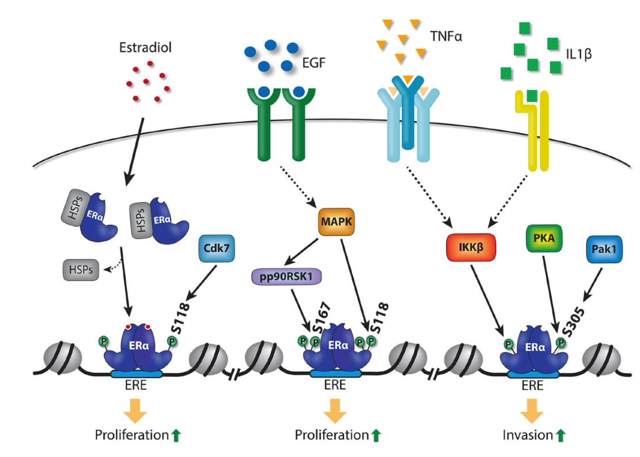
\includegraphics[width=0.5\textwidth]{../_resources/Screen_Shot_2022-11-18_at_11-59-02.png}
\caption{Screen Shot 2022-11-18 at 11-59-02.png}
\end{figure}

ER$\alpha$ ChIP-seq analyses of tumor samples revealed 484 ER common binding regions. ER$\alpha$-chromatin binding signal intensity is higher in tumors that progress towards a poorer prognosis and ultimately metastasize. The genes within 20 kilobases from the 484 ER-binding events exhibited elevated expression in the ER+ tumours, as compared to all other genes and were higher in ER+ tumours relative to ER- tumours. ER$\alpha$ ChIP seq revealed differential ER-binding events between patients with good outcome and patients with poor outcome or metastases.

\textbf{FOXA1} motifs were enriched in ER$\alpha$ binding regions of tam-resistant cells while \textbf{GATA} motifs were enriched in ER-binding events of tam-responsive cells. What is driving ER reprogramming?

Mitogen treatment of MCF7 cells (EGF, IL-6, TNF-a and IGF-I) reprogrammed ER-binding events

Distinct ER-binding profiles are associated with clinical outcome of breast cancer patients. These differential ER-binding profiles are for the most part mediated by FOXA1. Upregulation of growth factor pathways (along with ESR1 mutations and changes in cofactors levels) can influence ER binding reprogramming and the consequent change in gene expression profile fuels tumorigenesis and resistance to treatment of breast cancer cells. Since ER binding to DNA is for a good part dependent on FOXA1, targeting FOXA1, instead of ER might provide an opportunity for blocking ER transcriptional activity.

Half of all ER-binding regions overlap with a FoxA1-binding region. FOXA1 can open chromatin to ER. In addition, numerous ER-binding partners regulate ER transcriptional activity.

It was observed that transcriptional reprograming is present in Y537S and D538G mutants. Y537S and D538G mutants promote the transcription of a unique set of genes not induced by WT ER upon estrogen stimulation.

The FOXA1 motif was not significantly enriched in the mutant-selective binding sites, suggesting that FOXA1 may be less essential for mutant-specific ER DNA binding. E2-independent ER recruitment in the presence of the Y537S and D538G mutations, with a redistribution of 39\% and 49\% of the ER binding events for the Y537S and D538G mutations, respectively. CDK7 silencing impacted proliferation of both WT-ER and Y537S expressing cells.

In principle, if we find ER enhancer RNA promoting specific cancer genes, we can target it and selectively inhibiting it.
